%ADDING LAYERS

\documentclass[MASTER.tex]{subfiles} 
\begin{document} 

%=================================================%
\begin{frame}
	
\frametitle{Changing the plot type}
\vspace{-1cm}
\Large
\textbf{ggvis Layers}\\
\begin{itemize}
\item In ggplot2 you use \textbf{geom} functions to determine
the type of plot that you create
\item In ggvis you can use \texttt{layer} functions
\item N.B. Not all geoms are currently available as layers
\end{itemize}


\end{frame}
%=============================================================%
\begin{frame}[fragile]
	\frametitle{Layers}
	\large
So far, you seen two layer functions: \texttt{layer\_points()} and \texttt{layer\_histograms()}. There are many other layers, and they can be roughly categorised into two types:

\begin{itemize}
\item Simple, which include primitives like points, lines and rectangles.

\item Compound, which combine data transformations with one or more simple layers.
\end{itemize}
All layer functions use the plural, not the singular. 
\begin{quote}Think the verb, not the noun: I’m going to layer some points onto my plot.
\end{quote}
\end{frame}
%=================================================%
\begin{frame}
	\frametitle{Layers}

\begin{figure}
\centering
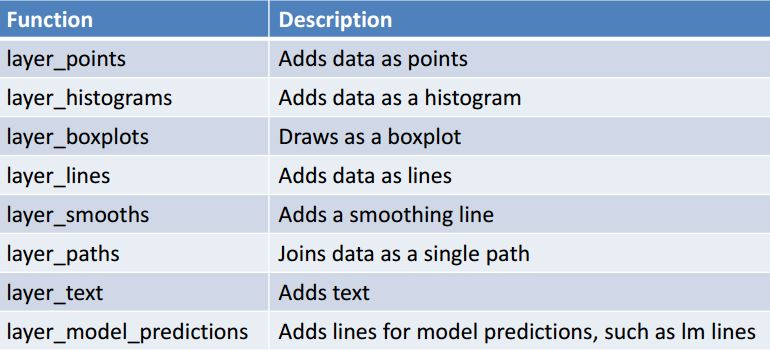
\includegraphics[width=1.19\linewidth]{images/ggvislayers}

\end{figure}

	
\end{frame}


%=================================================%
\begin{frame}[fragile]
\frametitle{Layers}
\Large
\vspace{-0.5cm}
\textbf{Simple layers}\\
There are five simple layers:

\begin{enumerate}
\item \textbf{Points} -\texttt{layer\_points}
\item \textbf{Paths} and \textbf{polygons}, - \texttt{layer\_paths()}.
\item \textbf{Filled Areas} - \texttt{layer\_ribbons()}
\item \textbf{Rectangles} - \texttt{layer\_rects()}
\item \textbf{Text} - \texttt{layer\_text()}\end{enumerate}

\end{frame}
%=================================================%
\begin{frame}[fragile]
	\Large
\textbf{1. Points, \texttt{layer\_points()}}
\\ properties: \texttt{x, y, shape, stroke, fill, strokeOpacity, fillOpacity}, and \texttt{opacity}.

\begin{framed}
\begin{verbatim}
mtcars  %>% 
   ggvis(~wt, ~mpg) %>% 
      layer_points()
\end{verbatim}
\end{framed}
\end{frame}
%=================================================%
\begin{frame}[fragile]
	\frametitle{Layers}
	\Large
\vspace{-0.4cm}
\textbf{2. Paths and polygons, layer\_paths()}.\\
\begin{framed}
	\begin{verbatim}
df <- data.frame(x = 1:10, 
       y = runif(10))

df %>% 
    ggvis(~x, ~y) %>% 
    layer_paths()
\end{verbatim}
\end{framed}
\end{frame}
%=================================================%
\begin{frame}[fragile]
	\frametitle{Layers}
\Large
If you supply a \texttt{fill}, you’ll get a polygon
\begin{framed}
	\begin{verbatim}
t <- seq(0, 2 * pi, length = 100)
df <- data.frame(x = sin(t), y = cos(t))

df %>% 
    ggvis(~x, ~y) %>% 
    layer_paths(fill := "red")
\end{verbatim}
\end{framed}
\end{frame}
%=================================================%
\begin{frame}[fragile]
	\frametitle{Layers}
	\Large
\textbf{3. Filled areas, \texttt{layer\_ribbons()}}\\ Use properties y and y2 to control the extent of the area.

\begin{framed}
	\begin{verbatim}
df <- data.frame(x = 1:10, 
    y = runif(10))
df %>% 
   ggvis(~x, ~y) %>% 
   layer_ribbons()
\end{verbatim}
\end{framed}

\end{frame}
%=================================================%
\begin{frame}[fragile]
	\frametitle{Layers}
\Large
\vspace{-1.4cm}
\begin{framed}
	\begin{verbatim}
 df %>% ggvis(~x, ~y + 0.1, 
             y2 = ~y - 0.1) %>% 
        layer_ribbons()
\end{verbatim}
\end{framed}
\end{frame}
%=================================================%
\begin{frame}[fragile]
	\frametitle{Layers}
\textbf{4. Rectangles, \texttt{layer\_rects()}}.\\ The location and size of the rectangle is controlled by the x, x2, y and y2 properties.

	\begin{framed}
		\begin{verbatim}
set.seed(1014)
df <- data.frame(x1 = runif(5), x2 = runif(5), 
         y1 = runif(5), y2 = runif(5))

df %>% ggvis(~x1, ~y1, 
           x2 = ~x2, y2 = ~y2, 
           fillOpacity := 0.1)  %>% 
       layer_rects()
\end{verbatim}
\end{framed}
\end{frame}

%=================================================%
\begin{frame}[fragile]
	\frametitle{Layers}
\textbf{5. Text, layer\_text().}.\\	
The \texttt{text} layer has many new options to control the apperance of the text: \begin{itemize}
\item \texttt{text} (the label), 
\item \texttt{dx} and \texttt{dy} (margin in pixels between text and anchor point), 
\item \texttt{angle} (rotate the text), 
\item \texttt{font} (font name) and fontSize (size in pixels),
\item \texttt{fontWeight} (e.g. bold or normal), 
\item \texttt{fontStyle} (e.g. italic or normal.)
\end{itemize}
\end{frame}

%=================================================%
\begin{frame}[fragile]
	\frametitle{Layers}
\Large
	\begin{framed}
		\begin{verbatim}
df <- data.frame(x = 3:1, 
        y = c(1, 3, 2), 
        label = c("a", "b", "c"))
        
df %>% ggvis(~x, ~y, text := ~label) 
   %>% layer_text()
\end{verbatim}
\end{framed}
\end{frame}
%=================================================%
\begin{frame}[fragile]
	\frametitle{Layers}
\vspace{-0.4cm}
\Large
	\begin{framed}
		\begin{verbatim}
df %>% 
  ggvis(~x, ~y, text := ~label) %>% 
  layer_text(fontSize := 50)
\end{verbatim}
\end{framed}
\end{frame}
%=================================================%
\begin{frame}[fragile]
	\frametitle{Layers}
\vspace{-0.4cm}
\Large
	\begin{framed}
		\begin{verbatim}
 df %>% 
     ggvis(~x, ~y, text := ~label) %>% 
     layer_text(angle := 45)
\end{verbatim}
\end{framed}
\end{frame}

%=================================================%
\begin{frame}[fragile]
	\frametitle{Layers}
\Large
\vspace{-1.5cm}
\textbf{Compound layers}\\
The four most common compound layers are:

\begin{enumerate}
\item \texttt{layer\_paths()}
\item \texttt{layer\_histograms()} 
\item \texttt{layer\_polygons()}
\item \texttt{layer\_smooths()}
\end{enumerate}
\end{frame}

%=================================================%
\begin{frame}[fragile]
	\frametitle{Layers}
	\Large
\texttt{layer\_lines()} which automatically orders by the x variable:
	\begin{framed}
		\begin{verbatim}
t <- seq(0, 2 * pi, length = 20)
df <- data.frame(x = sin(t), y = cos(t))

df %>% 
   ggvis(~x, ~y) %>% 
   layer_paths()
\end{verbatim}
\end{framed}
\end{frame}
%=================================================%
\begin{frame}[fragile]
\frametitle{Layers}
\Large
\textbf{Compound layers}\\
	\begin{framed}
		\begin{verbatim}
df %>% 
   ggvis(~x, ~y) %>% 
   layer_lines()
\end{verbatim}
\end{framed}
\end{frame}
%=================================================%
\begin{frame}[fragile]
\frametitle{Layers}
\Large
\texttt{layer\_lines()} is equivalent to \texttt{arrange()} + \texttt{layer\_paths()}:
\Large
\begin{framed}
\begin{verbatim}
 
df %>% 
   ggvis(~x, ~y) %>% 
   arrange(x) %>% 
   layer_paths()
\end{verbatim}
\end{framed}
\end{frame}
%=================================================%
\begin{frame}[fragile]
\frametitle{Layers}
\Large
\textbf{\texttt{layer\_histograms()} and \texttt{layer\_freqpolys()}}
\begin{itemize}
\item \texttt{layer\_histograms()} and \texttt{layer\_freqpolys()} which allows you to explore the distribution of continuous. 
\item Both layers first bin the data with \texttt{compute\_bin()} then display the results with either rects or lines.
\end{itemize}

\end{frame}
%=================================================%
\begin{frame}[fragile]
\frametitle{Layers}
\Large

\begin{framed}
\begin{verbatim}
mtcars  %>% 
   ggvis(~mpg) %>% 
   layer_histograms()
   
# Guessing width = 1 
# range / 24
\end{verbatim}
\end{framed}
\end{frame}
%=================================================%
\begin{frame}[fragile]
	\begin{framed}
		\begin{verbatim}
# Or equivalently
binned <- mtcars %>% compute_bin(~mpg) 

#  Guessing width = 1 
#  range / 24
binned   %>% ggvis(x = ~xmin_, 
         x2 = ~xmax_, 
         y2 = 0, y = ~count_, 
         fill := "black") %>% 
  layer_rects()
\end{verbatim}
\end{framed}
\end{frame}
%=================================================%
\begin{frame}[fragile]
\frametitle{Compound Layers}
\Large
\texttt{layer\_smooths()} fits a smooth model to the data, and displays predictions with a line. \\ It’s used to highlight the trend in noisy data:
\begin{framed}
\begin{verbatim}
mtcars   %>% 
   ggvis(~wt, ~mpg) %>% 
   layer_smooths()
\end{verbatim}
\end{framed}
\end{frame}
%=================================================%
\begin{frame}[fragile]
\large
You can control the degree of \textit{wiggliness} with the span parameter:
	\begin{framed}
		\begin{verbatim}
span <- input_slider(0.2, 1, value = 0.75)
mtcars  %>% 
  ggvis(~wt, ~mpg) %>% 
  layer_smooths(span = span)

\end{verbatim}
\end{framed}
\end{frame}
%=================================================%
\begin{frame}[fragile]
\Large
\textbf{Vignette}
\begin{itemize}
\item You can learn more about layers in the \textbf{layers} vignette.
\end{itemize}
\end{frame}

\end{document}
